\documentclass{article}
\usepackage[utf8]{inputenc} % LaTeX source encoded as UTF-8
\usepackage[margin=2cm]{geometry}
\usepackage{amssymb}
\usepackage{array}
\usepackage{tabularx}
\usepackage{tikz}


\title{Dotazník o~použitelnosti aplikace Virtuální historický průvodce}
\date{}
\begin{document}
\maketitle
\begin{figure}
\centering
  		
\includegraphics[width=10cm,keepaspectratio]{cvut-logo-bw.pdf}
\end{figure}
Prosíme o~vyplnění tohoto krátkého dotazníku pro účely testování použitelnosti prototypu aplikace Virtuální historicky průvodce. Dotazník je anonymní.



\subsection*{Demografie}

\begin{center}
\begin{tabular}{|c |c| c| c|c| c| c| }
 \hline
Váš věk & méně než 15 & 15 - 20 & 20 - 30 & 30 - 40 & 40 - 50 & 50 a více\\ 
  & $\square$ & $\square$ & $\square$ & $\square$ & $\square$ & $\square$\\ 
 \hline
\end{tabular}
\end{center}

\subsection*{Zájmy a technická zdatnost}

\begin{center}
\begin{tabular}{|c |c| c| c |c |c |}
 \hline
 & Ano & Spíš ano & Spíš ne & Ne\\ 
 \hline
 Už jste někdy používali technologie VR (virtuální realitu)? & $\square$ & $\square$& $\square$& $\square$\\ 
 \hline
 Vlastníte nějaké VR (SteamVR, Oculus, HTC Vive atd.)? & $\square$ & $\square$& $\square$& $\square$\\ 
 \hline
 Pracujete pravidelně na PC? & $\square$ & $\square$& $\square$& $\square$\\ 
 \hline
 Hrajete počítačové hry? & $\square$ & $\square$& $\square$& $\square$\\ 
 \hline
 Zajímá vás historie? & $\square$ & $\square$& $\square$& $\square$\\ 
 \hline
 Zajímá vás stará architektura? & $\square$ & $\square$& $\square$& $\square$\\ 
 \hline
 Cestujete rádi po historických místech? & $\square$ & $\square$& $\square$& $\square$\\ 
 \hline
\end{tabular}
\end{center}



\subsection*{Hodnocení aplikace}

\begin{table}[htb]
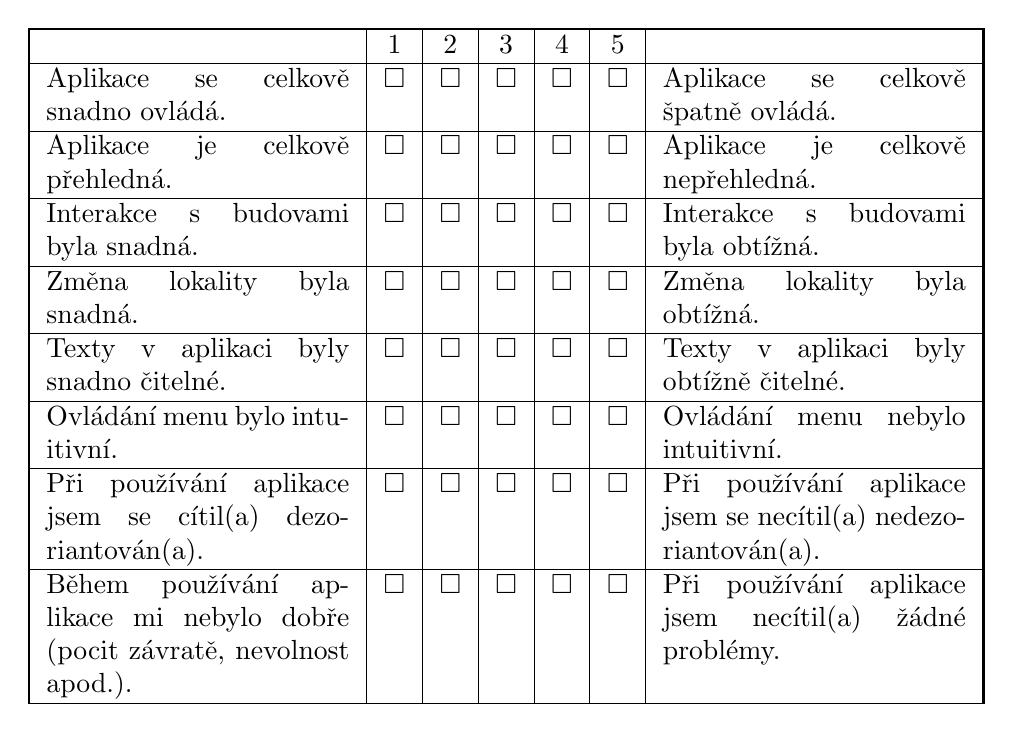
\begin{tikzpicture}
\node (table) [inner sep=0pt] {
\begin{tabularx}{\textwidth}{|X|c|c|c|c|c|X|}
  \hline
   & 1  & 2 & 3 & 4 & 5 &\\
  \hline
  Aplikace se celkově snadno ovládá. & $\square$ & $\square$ & $\square$ & $\square$ & $\square$ &  Aplikace se celkově špatně ovládá.\\
  \hline
 Aplikace je celkově přehledná.  & $\square$ & $\square$ & $\square$ & $\square$ & $\square$ & Aplikace je celkově nepřehledná. \\
  \hline
Interakce s~budovami byla snadná.  & $\square$ & $\square$ & $\square$ & $\square$ & $\square$ & Interakce s~budovami byla obtížná.\\
  \hline
Změna lokality byla snadná.  & $\square$ & $\square$ & $\square$ & $\square$ & $\square$ & Změna lokality byla obtížná.\\
  \hline
Texty v~aplikaci byly snadno čitelné.  & $\square$ & $\square$ & $\square$ & $\square$ & $\square$ & Texty v~aplikaci byly obtížně čitelné.\\
  \hline
Ovládání menu bylo intuitivní.  & $\square$ & $\square$ & $\square$ & $\square$ & $\square$ & Ovládání menu nebylo intuitivní.\\
  \hline
Při používání aplikace jsem se cítil(a) dezoriantován(a).  & $\square$ & $\square$ & $\square$ & $\square$ & $\square$ & Při používání aplikace jsem se necítil(a) nedezoriantován(a).\\
  \hline
Během používání aplikace mi nebylo dobře (pocit závratě, nevolnost apod.). & $\square$ & $\square$ & $\square$ & $\square$ & $\square$ & Při používání aplikace jsem necítil(a) žádné problémy.\\
\end{tabularx}
};
\draw (table.north west) rectangle (table.south east);
\end{tikzpicture}
\end{table}
\thispagestyle{empty}
\end{document}